\section{Results}
\label{sec:results}


\begin{figure}
\begin{center}
\begin{tabular}{cc}
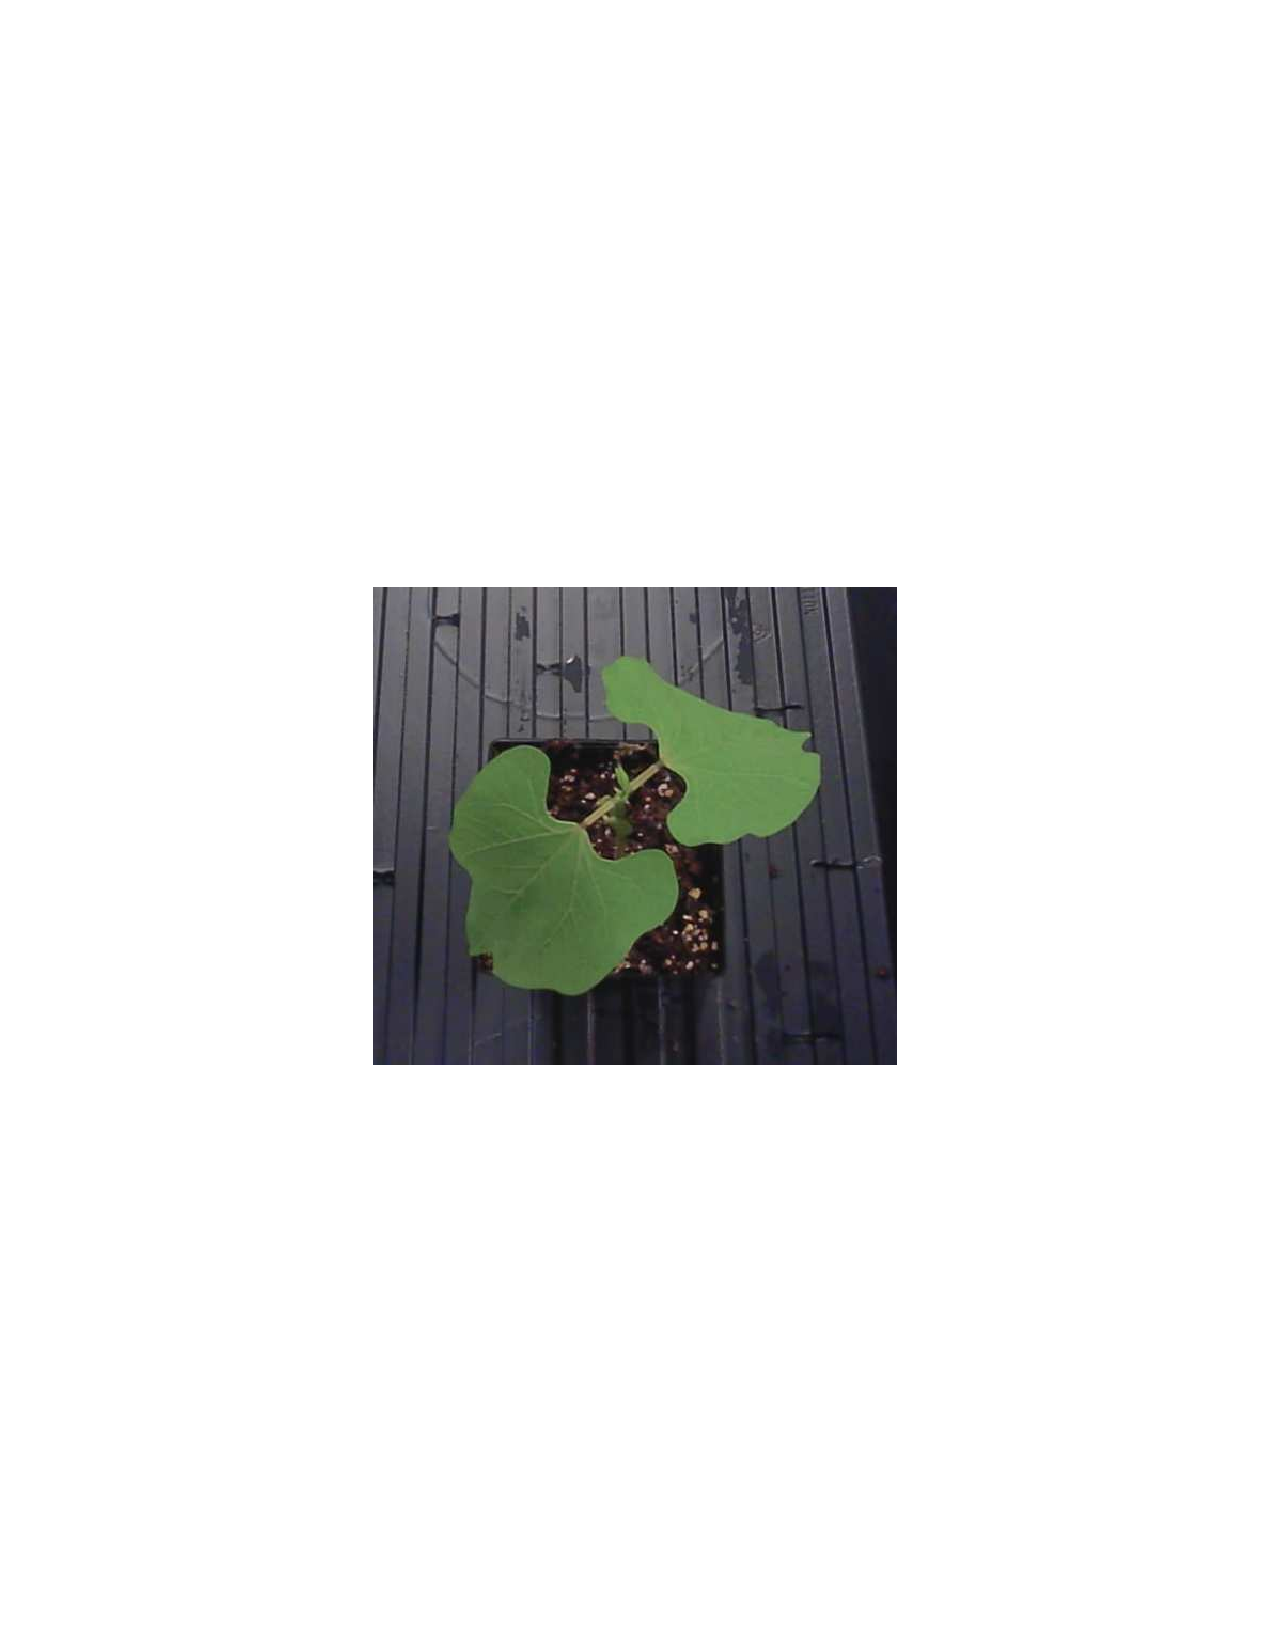
\includegraphics[trim=190 280 190 290,clip,width=0.48\linewidth]{Figures/beanColor} &
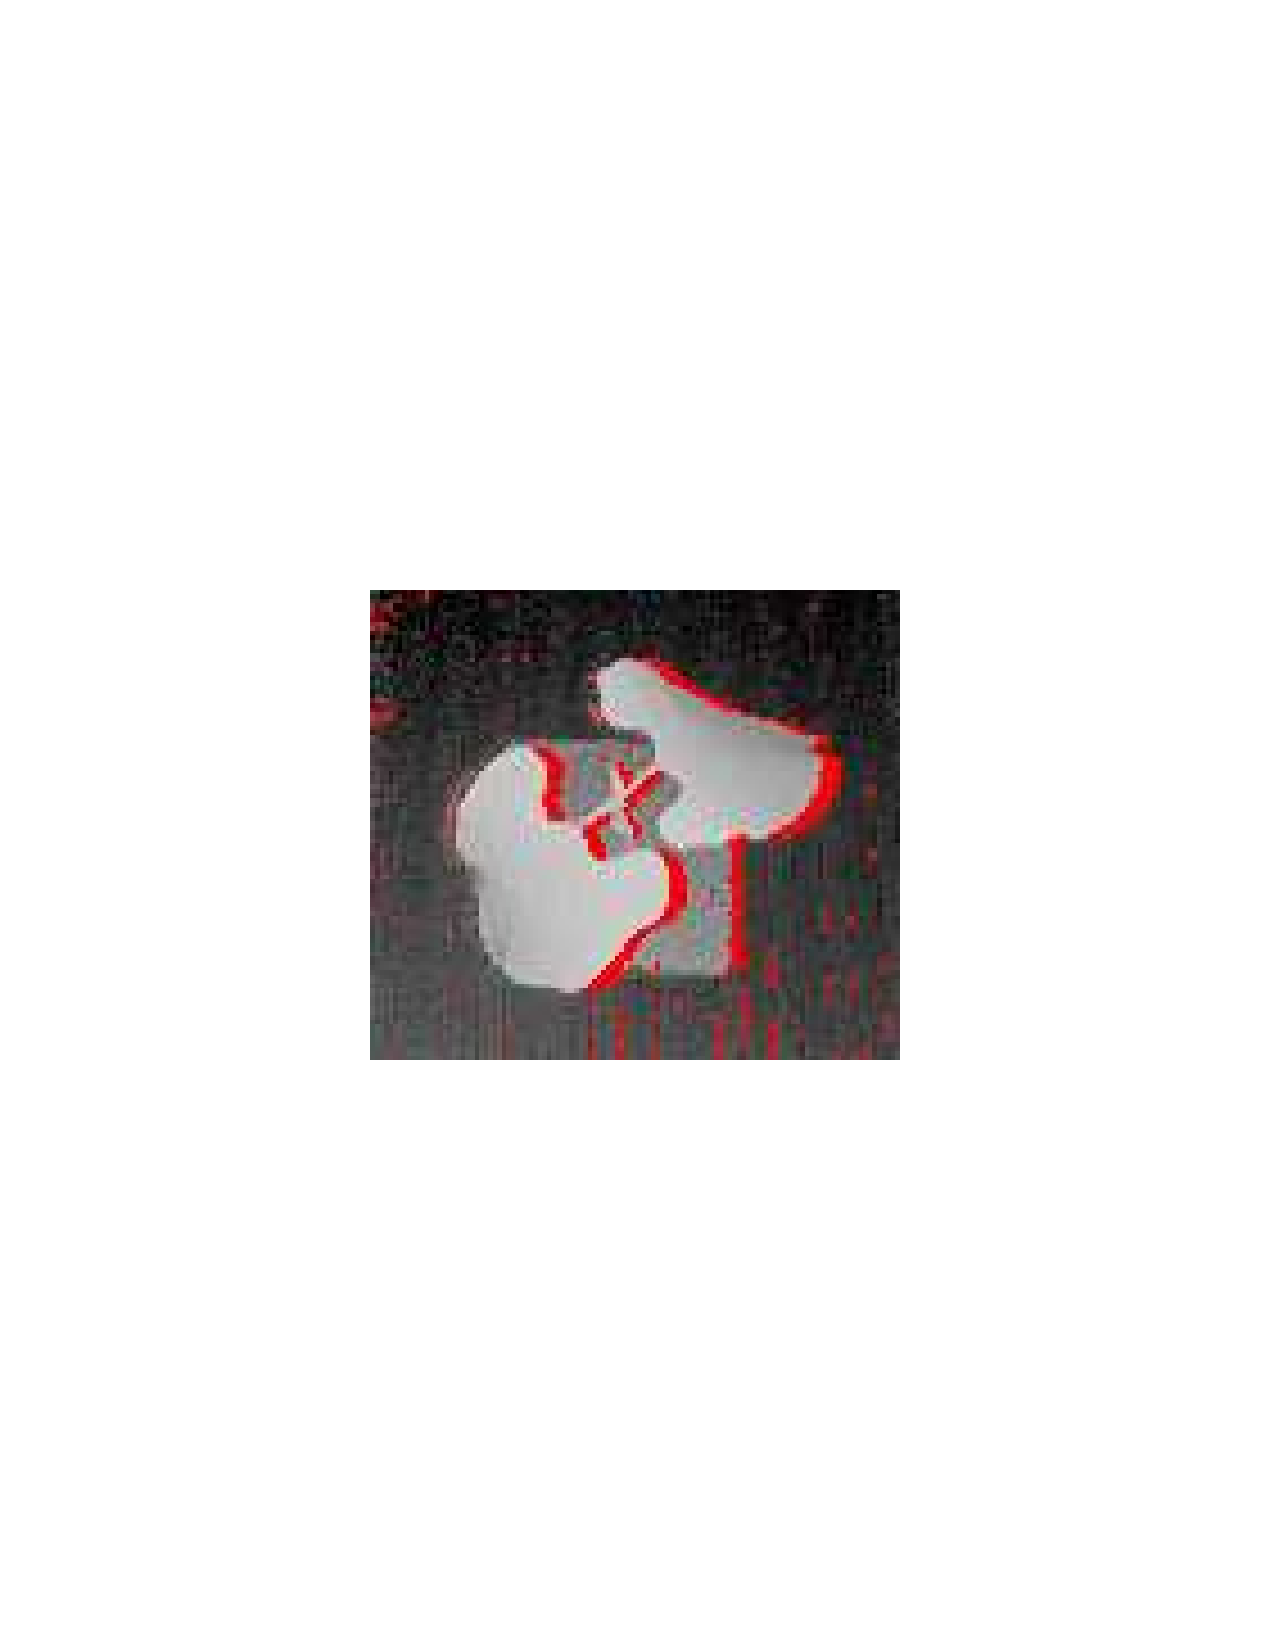
\includegraphics[trim=190 280 190 290,clip,width=0.48\linewidth]{Figures/beanDepth} \\
($a$) & ($b$) \\
%Put bead SLIC and boundary here:
($c$) & ($d$) \\
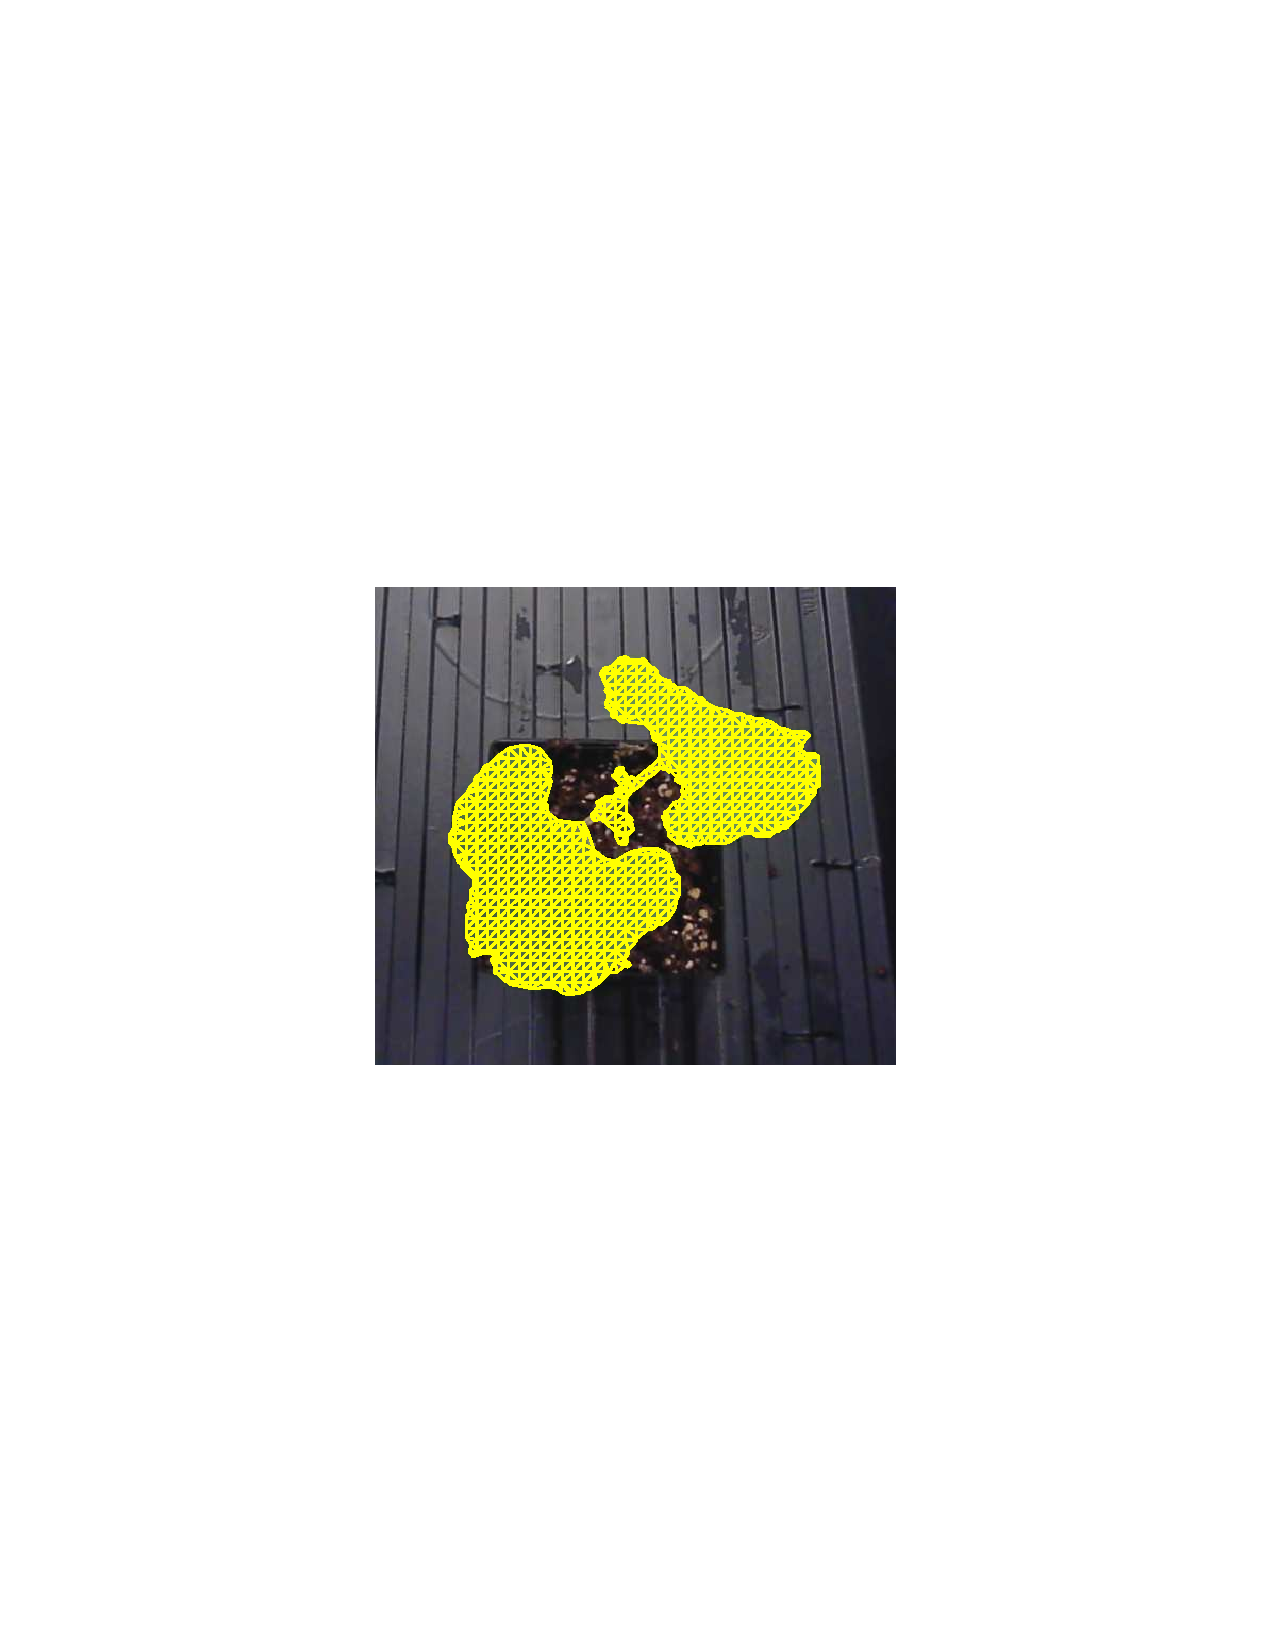
\includegraphics[trim=190 280 190 290,clip,width=0.48\linewidth]{Figures/beanColorMesh} &
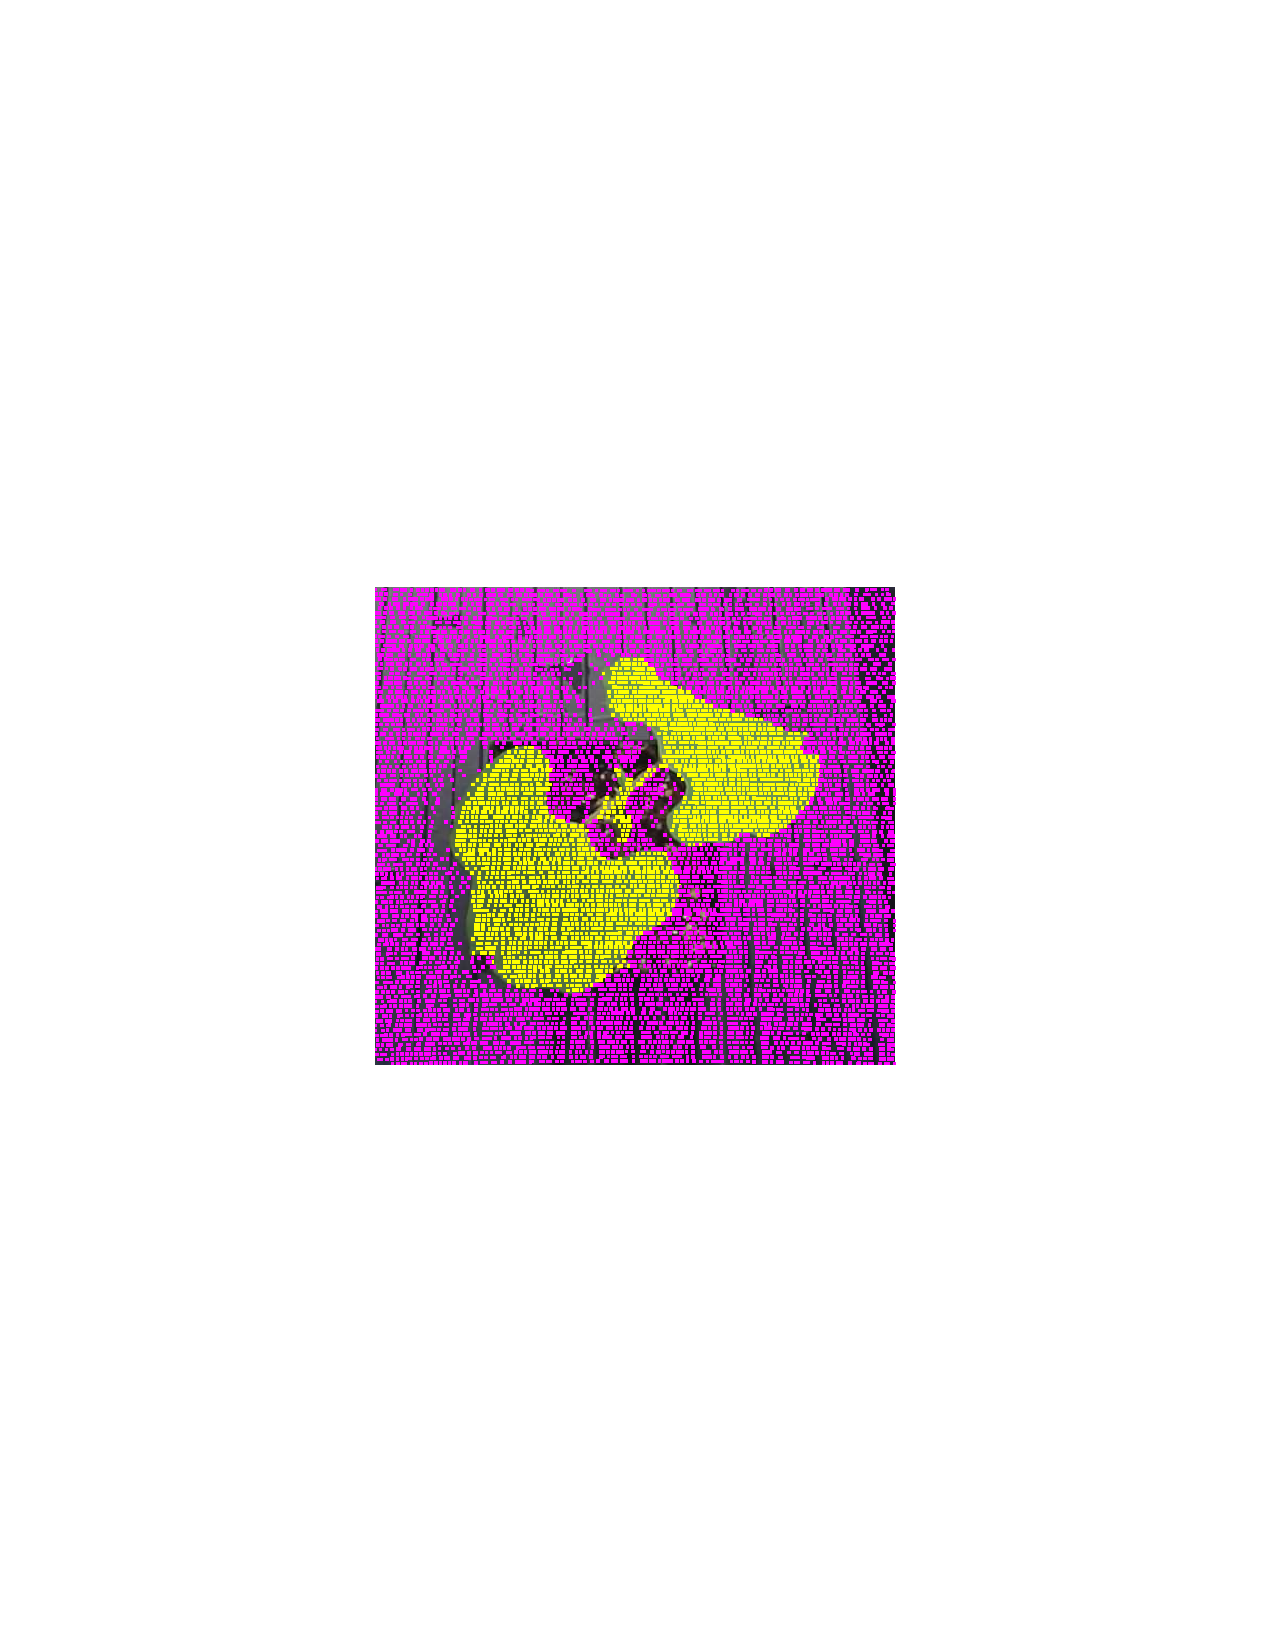
\includegraphics[trim=190 280 190 290,clip,width=0.48\linewidth]{Figures/beanPointsOnLeaves} \\
($e$) & ($f$) \\
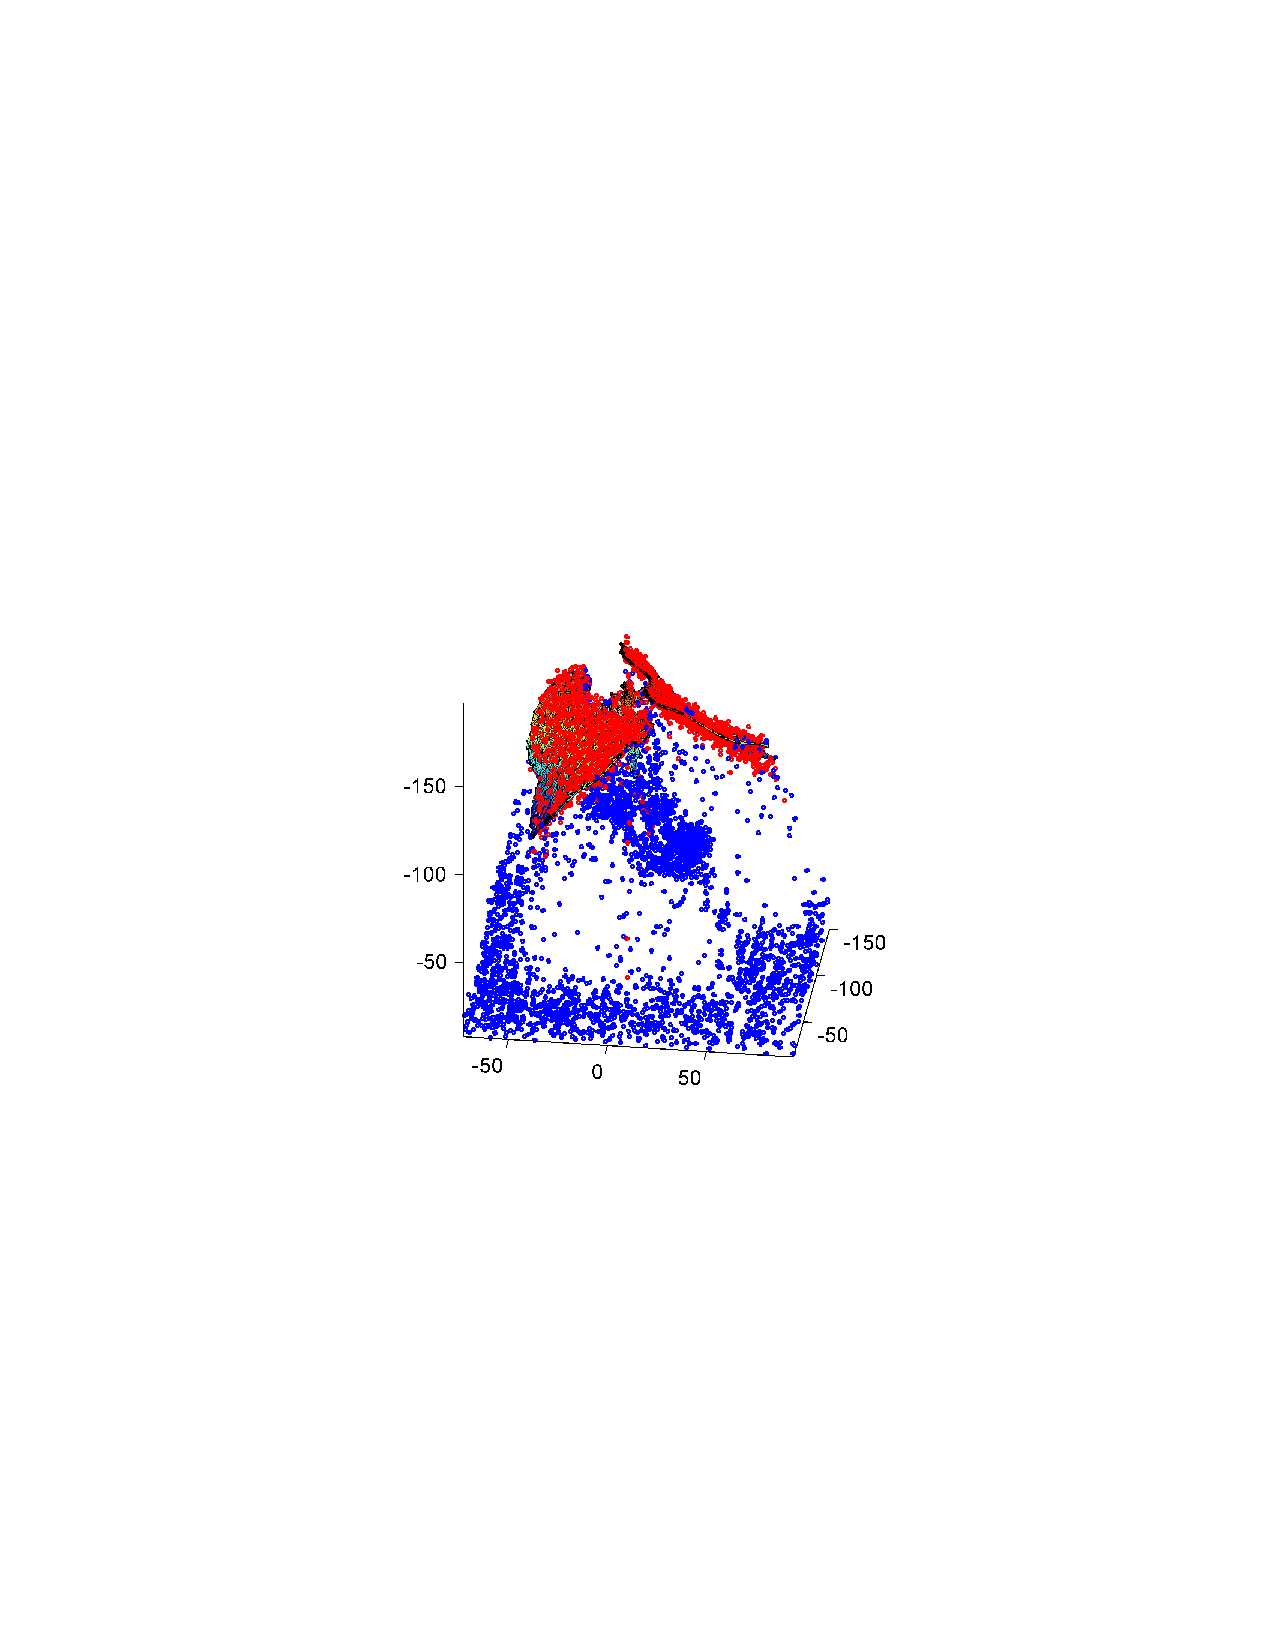
\includegraphics[trim=190 280 190 290,clip,width=0.48\linewidth]{Figures/bean3DMeshPlusPoints} &
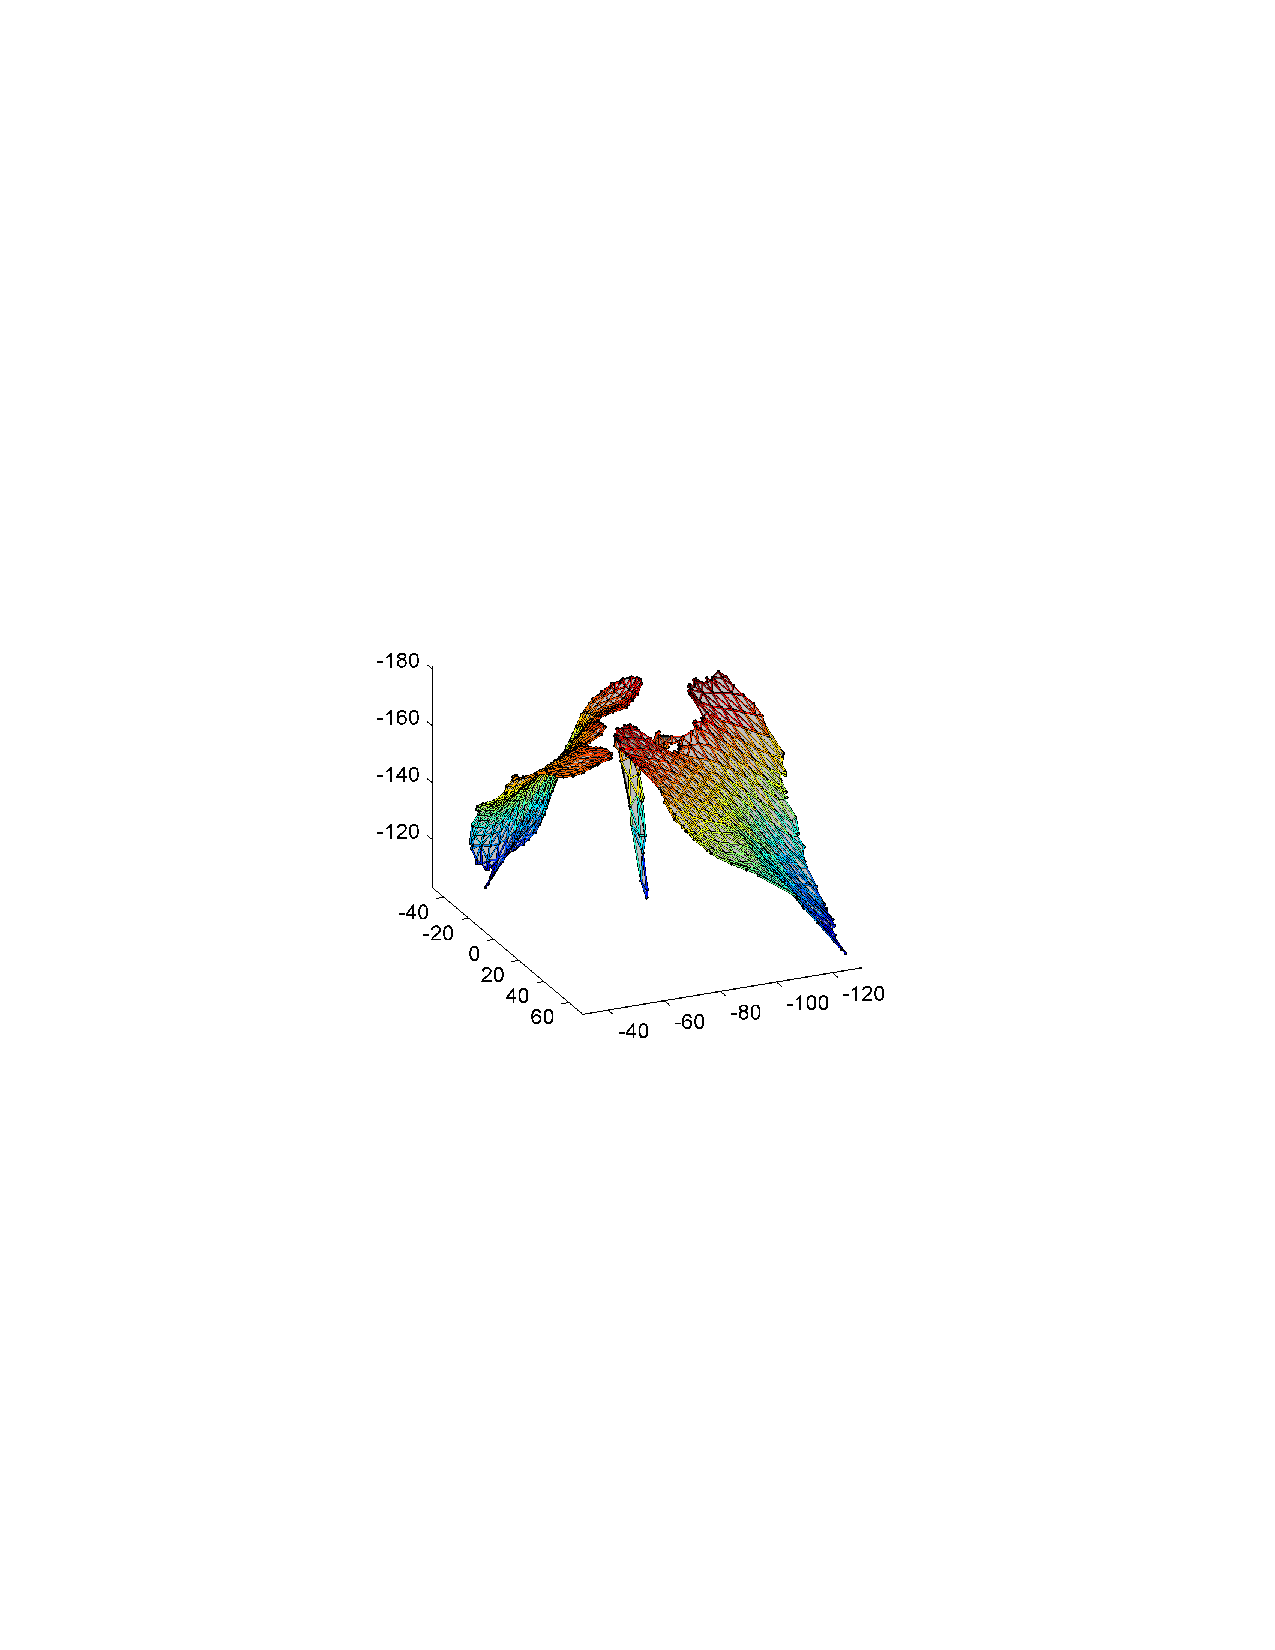
\includegraphics[trim=190 280 190 290,clip,width=0.48\linewidth]{Figures/bean3DMesh} \\
($g$) & ($h$) \\
\end{tabular}
\end{center}
   \caption{($a$) Color image.  ($b$) Depth image.  White pixels are those that are automatically masked out due to being not visible in the color image.}
\label{fig:sigmainterframe}
\end{figure}



